\documentclass[aspectratio=169,
hyperref={colorlinks,urlcolor=blue}
]{beamer}


%\usetheme{Pittsburgh}
\usetheme{default}
\usepackage{colortbl}%colored tables
%For using helvetica font:
\usepackage[scaled]{helvet}
\usepackage[T1]{fontenc}
\renewcommand\familydefault{\sfdefault}
\urlstyle{same} %sets the fonts for urls
\usepackage{pdfpages}
\usepackage{siunitx}
\usepackage{caption}
\usepackage{pifont}%for dings
\usepackage{pgfplots}%for 3d plotting
\pgfplotsset{compat = newest}
\usepackage{mathtools}%box in align env \Aboxed
\usepackage[american,smartlabels]{circuitikz}%for drawing circuits
\usepackage{multimedia}
\usepackage{animate}
\usepackage{xcolor}


\usetikzlibrary{arrows}
\usetikzlibrary {3d} 
\usetikzlibrary{decorations.markings, math}
\usetikzlibrary{intersections, pgfplots.fillbetween}
\usetikzlibrary {shapes.geometric} 


%\definecolor{myblue}{RGB}{5, 34, 150}
\definecolor{myblue2}{RGB}{5, 34, 150}
\definecolor{myblue}{RGB}{0,36,82}
\definecolor{myred}{RGB}{207, 2, 13}
\definecolor{mygreen}{RGB}{0, 158, 11}
\definecolor{myyellow}{RGB}{220,220,0}
\definecolor{qblue}{RGB}{0,36,82}
\definecolor{qgold}{RGB}{250,189,15}
\definecolor{qred}{RGB}{185,14,49}
\definecolor{cblue}{rgb}{0.13, 0.67, 0.8}
\definecolor{corange}{rgb}{0.8, 0.34, 0.0}
\definecolor{cpurple}{rgb}{0.54, 0.29, 0.42}

%%%%%%%%%%%% General settings
\setbeamercolor{frametitle}{fg=black}
\setbeamercolor{title}{fg=black}
\setbeamercolor{author}{fg=myblue2}

\beamertemplatenavigationsymbolsempty %no navigation controls at bottom of slides
%\setbeamertemplate{footline}[frame number]
\usefonttheme{professionalfonts} 
\setbeamerfont{title}{series=\bfseries,parent=structure}
\setbeamerfont{frametitle}{series=\bfseries,parent=structure}

%%%%%%%%%%%%Lists
\setbeamertemplate{itemize item}[circle] %{\color{myblue}$\circ$}
\setbeamertemplate{itemize subitem}{\color{myblue2}$\circ$}
\setbeamertemplate{itemize subsubitem}{\color{myblue2}$\cdot$}
\setbeamercolor{itemize item}{bg=myblue2,fg=myblue2}
\setbeamercolor{enumerate item}{bg=myblue2,fg=myblue2}
%%%%%%%%%%%%%%%%%%%%%%%%%%%%

%%%%%%%%%%%%Blocks
\setbeamertemplate{blocks}[rounded]
%Default block
\setbeamercolor{block title}{bg=myblue2, fg=white}
\setbeamercolor{block body}{bg=myblue2!10}
\setbeamerfont{block body}{size=\scriptsize}
\setbeamerfont{block title}{size=\scriptsize}
%Alert block
\setbeamercolor{block title alerted}{bg= myblue2, fg=white}
\setbeamercolor{block body alerted}{bg=myblue2!10}
\setbeamerfont{block body alerted}{size=\scriptsize}
\setbeamerfont{block title alerted}{size=\scriptsize}
%example block
\setbeamercolor{block title example}{bg=mygreen, fg=white}
\setbeamercolor{block body example}{bg=mygreen!10}
\setbeamerfont{block body example}{size=\scriptsize}
\setbeamerfont{block title example}{size=\scriptsize}
%%%%%%%%%%%%%%%%55


%%%%%%%%%%%%Figures and captions
\captionsetup{font=scriptsize,labelfont=scriptsize}
%\setbeamertemplate{caption}{\raggedright\insertcaption\par}
\newenvironment{capfig}[3]{\begin{figure}\includegraphics[width=#1\textwidth]{#2}\caption*{\textit{#3}}\end{figure}}{}

%\makeatother
%\setbeamertemplate{footline}
%{
%  \leavevmode%
%  \hbox{%
%  \begin{beamercolorbox}[wd=.4\paperwidth,ht=2.25ex,dp=1ex,center]{author in head/foot}%
%    \usebeamerfont{author in head/foot}\insertshortauthor
%  \end{beamercolorbox}%
%  \begin{beamercolorbox}[wd=.6\paperwidth,ht=2.25ex,dp=1ex,center]{title in head/foot}%
%    \usebeamerfont{title in head/foot}\insertshorttitle\hspace*{3em}
%    \insertframenumber{} / \inserttotalframenumber\hspace*{1ex}
%  \end{beamercolorbox}
%  }%
%  \vskip0pt%
%}
%\makeatletter

\makeatother
\setbeamertemplate{footline}
{
  \leavevmode%
  \hbox{%
\begin{beamercolorbox}[wd=.27\paperwidth,ht=2.25ex,dp=1ex,center]{author in head/foot}%
    \color{black}{\insertinstitute}
\end{beamercolorbox}
  \begin{beamercolorbox}[wd=.27\paperwidth,ht=2.25ex,dp=1ex,center]{author in head/foot}%
    \color{black}{\inserttitle}
  \end{beamercolorbox}%
  \begin{beamercolorbox}[wd=.27\paperwidth,ht=2.25ex,dp=1ex,center]{title in head/foot}%
    \color{black}{\insertshortauthor}
  \end{beamercolorbox}
  \begin{beamercolorbox}[wd=.27\paperwidth,ht=2.25ex,dp=1ex,center]{title in head/foot}%
    \hspace{.28\paperwidth}\color{black} \insertframenumber{} / \inserttotalframenumber\hspace*{1ex}
  \end{beamercolorbox}
  }%
  \vskip0pt%
}
\makeatletter

\setbeamertemplate{title page}
{
  \begin{tikzpicture}[remember picture,overlay]
    \def\barh{4}%15
  
    \draw[color=myblue2,line width=\barh] ([yshift=-0.5*\barh]current page.north west) -- ([yshift=-0.5*\barh,xshift=-0.67\paperwidth]current page.north east);
    \draw[color=myblue2,line width=\barh] ([yshift=-0.5*\barh,xshift=-0.67\paperwidth]current page.north east) -- ([yshift=-0.5*\barh,xshift=-0.34\paperwidth]current page.north east);
    \draw[color=myblue2,line width=\barh] ([yshift=-0.5*\barh,xshift=-0.34\paperwidth]current page.north east) -- ([yshift=-0.5*\barh]current page.north east); 
  
    \draw[color=myblue2,line width=\barh] ([yshift=0.5*\barh]current page.south west) -- ([yshift=0.5*\barh,xshift=-0.67\paperwidth]current page.south east);
    \draw[color=myblue2,line width=\barh] ([yshift=0.5*\barh,xshift=-0.67\paperwidth]current page.south east) -- ([yshift=0.5*\barh,xshift=-0.34\paperwidth]current page.south east);
    \draw[color=myblue2,line width=\barh] ([yshift=0.5*\barh,xshift=-0.34\paperwidth]current page.south east) -- ([yshift=0.5*\barh]current page.south east);
    %\node[left] at (current page.east) {
    %
\includegraphics[scale=0.1]{figures/coverpage}
    %};
  \end{tikzpicture}
  
  \usebeamerfont{title}\usebeamercolor[fg]{title}\inserttitle\par
  \usebeamerfont{subtitle}\usebeamercolor[fg]{subtitle}\insertsubtitle\par
  \vspace{2cm}
  \usebeamerfont{author}\usebeamercolor[fg]{author}\insertauthor\par
  \usebeamerfont{institute}\usebeamercolor[fg]{author}\insertinstitute\par
  \usebeamercolor[fg]{author}\par
  \usebeamercolor[fg]{titlegraphic}\inserttitlegraphic

} 

\setbeamertemplate{frametitle}{%
    \nointerlineskip%
        \par\hspace*{-\dimexpr0.5\paperwidth-0.5\textwidth}\textcolor{myblue2}{\rule{0.33\paperwidth}{6pt}}\textcolor{myblue2}{\rule{0.33\paperwidth}{6pt}}\textcolor{myblue2}{\rule{0.34\paperwidth}{6pt}} 
    \begin{beamercolorbox}[wd=\paperwidth,ht=0.75cm,dp=0.6ex]{frametitle}
        \hspace*{0.5cm}\strut\usebeamerfont{frametitle}\insertframetitle\strut
        %\hrule
    \end{beamercolorbox}%
    %%Line below:
%\par\hspace*{-\dimexpr0.5\paperwidth-0.5\textwidth}\textcolor{myblue}{\rule{\paperwidth}{0.4pt}}
     % <-- calculation of left margin width + rule
     %\textcolor{red}{\noindent\rule{\paperwidth}{2pt}}
}


%%%%%%%%%%%%Frame templates

%Slide with title
\newenvironment{titleframe}[1]
{\begin{frame}\frametitle{#1}\end{frame}}
{}

%Slide with title and itemize list:
\newenvironment{bulletframe}[1]
{\begin{frame}{#1} \itemize}
{\enditemize \end{frame}}

%Slide with two columns 50/50
\newenvironment{twocolframe}[3]
{\begin{frame}{#1}
 \begin{columns}[T]
 \column{0.5\textwidth}#2
 \column{0.5\textwidth}#3
 \end{columns}\end{frame}}{}

%Slide with two columns 60/40 <<<<<<<<<<<<<<<<<<<<<<  This one!
\newenvironment{twocolframesf}[3]
{\begin{frame}{#1}
 \begin{columns}[T]
 \column{0.6\textwidth}#2
 \column{0.4\textwidth}#3
 \end{columns}\end{frame}}{}
 
%Slide with two columns 70/30
\newenvironment{twocolframest}[3]
{\begin{frame}{#1}
 \begin{columns}[T] 
 \column{0.7\textwidth}#2
 \column{0.3\textwidth}#3
 \end{columns}\end{frame}}{} 
 
%Slide with two columns 40/60
\newenvironment{twocolframefs}[3]
{\begin{frame}{#1}
 \begin{columns}[T] 
 \column{0.4\textwidth}#2
 \column{0.6\textwidth}#3
 \end{columns}\end{frame}}{}
 
%Slide with two columns 70/30
\newenvironment{twocolframets}[3]
{\begin{frame}{#1}
 \begin{columns}[T] 
 \column{0.3\textwidth}#2
 \column{0.7\textwidth}#3
 \end{columns}\end{frame}}{} 

 
%Colloquium speaker (title, abstract, picture file, speaker name)
\newenvironment{colloquium}[5]
{
\begin{frame}{Colloquium: Friday 1:30pm in Stirling A}
\begin{columns}[T] 
 \column{0.8\textwidth}
 \textbf{#1}\\
 #2
 \column{0.2\textwidth}
 \capfig{#3}{#4}{#5}
 \end{columns}
\end{frame}
}
{} 

%%%%%%%%%%%%%Set Hyperref colors


\hypersetup{
  colorlinks=true,
  linkcolor=blue,    
  urlcolor=blue,     
  citecolor=blue      
}
%%%%%%%%%%%%%TOC bolding
\setbeamerfont{section in toc}{series=\bfseries}



%Frames:
% \twocolframesf 60/40 (fs, st, ts) 
% \titleframe
% bulletframe


%%%%%%%%%%%%%%%%%%%%%%%%%
%%%%%% START OF PRESENTATION %%%%%%
%%%%%%%%%%%%%%%%%%%%%%%%%

\title{Rotational Dynamics}
\institute{Describing angular statics and dynamics}
\author{Building Models to Describe our World}


\begin{document}
	
%%%%%%%%%%%%%%%%%%%%%%%%%
%%%%%% Title slide %%%%%%
%%%%%%%%%%%%%%%%%%%%%%%%%
\begin{frame}
\titlepage
\thispagestyle{empty}

\begin{textblock*}{5cm}(11cm,4cm)
    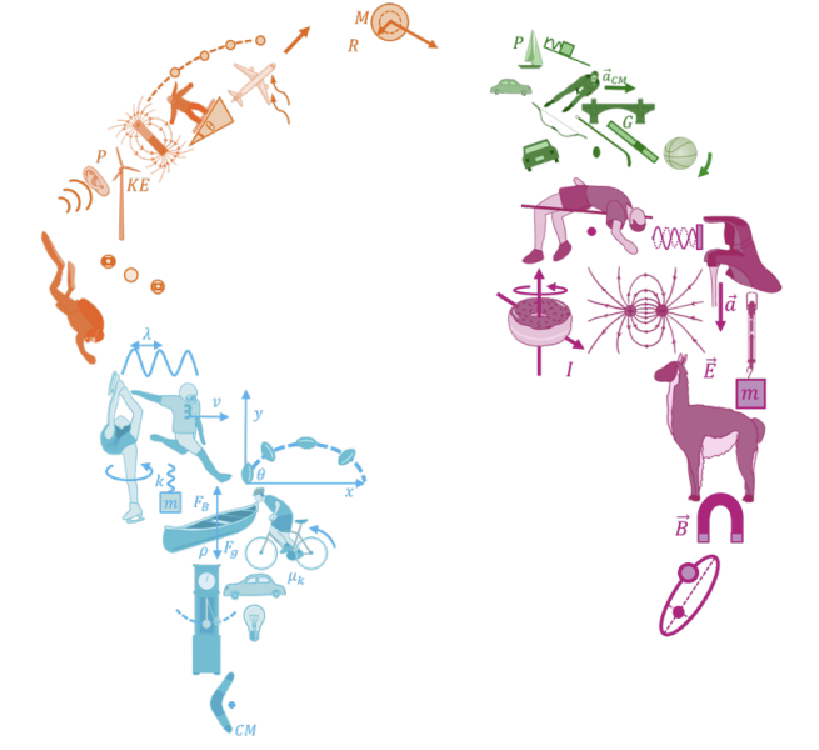
\includegraphics[width=4cm]{../figures/BMDW/logo}
\end{textblock*}

\end{frame}

%%%%%%%%%%%%%TOC

\twocolframe{Outline}
{\tableofcontents[sections=1-2, subsectionstyle=show/show]}
{\tableofcontents[sections=3, subsectionstyle=show/show]}

%%%%%%%%%%%%%%%%%%%%%%%%%











%%%%%%%%%%%%%%%%%%%%%%%%%%%%%%%%
\section{Angular Quantities and Torque}
\label{sec:angulartquantitesandtorque}
\title{Angular Quantities and Torque}
\institute{Describing Angular Statics and Dynamics}
\author{\insertsubsection}


%%%%%%%%%%%%%%%%%%%%%%%%%
\begin{frame}
\titlepage
\thispagestyle{empty}
\end{frame}

%%%%%%%%%%%%%%%%%%%%%%%%%








%%%%%%%%%%%%%%%%%%%%%%%%%%%%%%%%%%%%%%%%%%%%%%%

\begin{frame}{Context}
We started with $\sum \vec F=m \vec a$, and then:
\begin{itemize}
\item Used $\sum \vec F=m \vec a$ as is.
\item Took $\int (\sum \vec F=m \vec a ) \cdot d\vec l$ to define work and energy.
\item Took $\int (\sum \vec F=m \vec a ) dt$ to introduce impulse and momentum.
\end{itemize}
This week, we do:
\begin{align*}
\vec r \times \Bigl(\sum \vec F=m \vec a \Bigr)
\end{align*}
in order to model rotating systems.
\end{frame}


%%%%%%%%%%%%%%%%%%%%%%%%%%%%%%%%
\subsection{Describing rotating things}
\label{subsec:describingrotatingthings}
\twocolframesf{Describing things that rotate in 2D}
{
\vspace{-0.25cm}
\begin{itemize}
\item Recall that we can describe circular motion using linear or angular quantities:
\begin{align*}
s&=R\theta\\
v&=R\omega\\
a_T&=\alpha R
\end{align*}
\item The angular quantities are \textbf{related to the tangential} linear quantities. The acceleration also has a radial component:
\begin{align*}
a_R=\frac{v^2}{R}=\omega^2 R
\end{align*}
due to the \textbf{change of the direction} of the velocity vector (not its magnitude).
\end{itemize}
}
{
\begin{center}
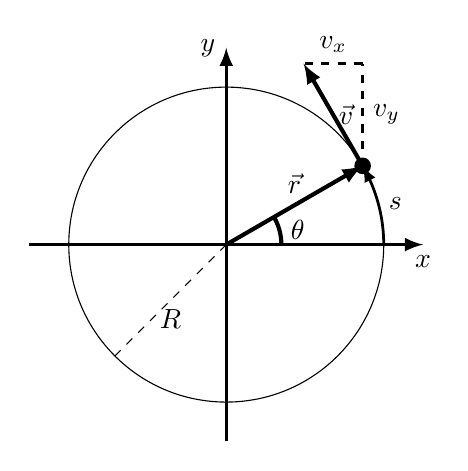
\begin{tikzpicture}[scale=1]
\tikzmath{
\R=2;
\th=30;
\Px=\R*cos(\th);
\Py=\R*sin(\th);
\vel=1.5;
\vx=-\vel*sin(\th);
\vy=\vel*cos(\th);
}
\scalebox{1}{

\coordinate (P) at (\Px,\Py);

\draw[-latex, line width=1.25pt] (-1.25*\R,0) -- (1.25*\R,0) node[below]{$x$}; 
\draw[-latex, line width=1.25pt] (0,-1.25*\R) -- (0,1.25*\R) node[left]{$y$};

\draw (0,0) circle (\R); 
\fill (P) circle(3pt);
\draw[-latex, line width = 1.5] (0,0) -- (P) node[midway,above] {$\vec r$};
\draw[line width = 1.5] (0.7,0) arc (0:\th:0.7) node[midway,right]{$\theta$};
\draw[-latex, line width = 1.5] (P) -- +(\vx,\vy) node[midway,right=-2pt] {$\vec v$};
\draw[dashed, line width = 1.] (P) -- +(0,\vy) node[midway,right] {$v_y$};
\draw[dashed, line width = 1.] ($(P) +(0,\vy)$) -- +(\vx,0) node[midway,above] {$v_x$};

\draw[dashed] (0,0) --+(225:\R) node[midway,below]{$R$};

\draw[-latex, line width=1] (\R,0) arc (0:\th:\R) node[midway,right]{$s$};

}
\end{tikzpicture}
\captionof*{figure}{\textit{Variables to describe circular motion.}}
\end{center}
}


%%%%%%%%%%%%%%%%%%%%%%%%%%%%%%%%
\twocolframesf{Describing things that rotate in 3D}
{
\begin{itemize}
\item In general, things rotate in a circle:
\begin{itemize}
\item About an axis (defining a normal plane).
\item In a specific direction around the axis.
\item With a specific amplitude/speed/acceleration.
\end{itemize}
\item Use ``axial/pseudo vectors'' to specify:
\begin{itemize}
\item $\vec \theta$, angular displacement.
\item $\vec \omega$, angular velocity.
\item $\vec \alpha$, angular acceleration.
\end{itemize}
with magnitudes given by the same value as in 2D, and \textbf{direction given by the  ``right hand rule for axial vectors''}.
\end{itemize}
}
{
\begin{center}
\begin{tikzpicture}[scale=1]

\scalebox{1}{

\node at (0,0) {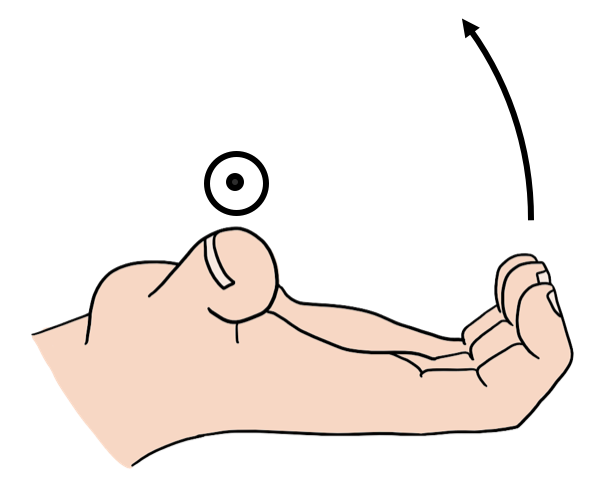
\includegraphics[scale=0.5]{../figures/RotationalDynamics/righthandruleaxial}};
\node at (-0.5,1.2) {$\vec \omega$};

}
\end{tikzpicture}
\captionof*{figure}{\textit{The right-hand rule for axial vectors is used to define the direction of a vector associated with rotation. The thumb is parallel to the axis of rotation and the fingers curl in the direction of rotation.}}
\end{center}
}


%%%%%%%%%%%%%%%%%%%%%%%%%%%%%%%%


%%%%%%%%%%%%%%%%%%%%%%%%%%%%%%%%
\subsection{Angular Vectors}
\label{subsec:angularvectors}
\twocolframesf{Angular vectors from linear vectors}
{
\begin{itemize}
\item Need to be able to describe rotation about any axis (not just $x,y,z$).
\item The angular vectors are related to the linear ones:
\begin{align*}
\vec \omega&=\frac{1}{r^2}\vec r \times \vec v\\
\vec \alpha&=\frac{1}{r^2}\vec r \times \vec a
\end{align*}
\item The vector, $\vec r$, is perpendicular to the axis of rotation and goes \textbf{from the axis of rotation to the particle's position}.
\end{itemize}
}
{
\begin{center}
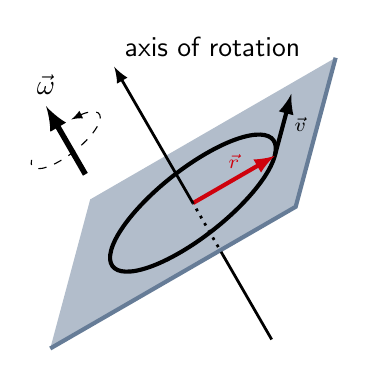
\begin{tikzpicture}[scale=1]
\tikzmath{
\R=1.2;
}

\scalebox{1}{
\begin{scope}[rotate=30]

%angular velocity vector
\draw[-latex, line width=2] (-1,1,0) -- +(0,1,0) node[above]{$\vec \omega$};
%circle around omega
\begin{scope}[canvas is xz plane at y=1.5]
\draw[latex-,dashed] (-1,-0.5) arc(-90:180:0.5);
\end{scope}

\begin{scope}[canvas is xz plane at y=0]
%the plane
\fill[myblue!30] (-1.5*\R,-1.5*\R) -- (1.5*\R,-1.5*\R) -- (1.5*\R,1.5*\R) -- (-1.5*\R,1.5*\R) --cycle;
\draw[line width=1.5,color=myblue!60]  (1.5*\R,-1.5*\R) -- (1.5*\R,1.5*\R)-- (-1.5*\R,1.5*\R);
\draw[line width=1.5] (0,0) circle(\R);
\draw[-latex,line width=1.5,color=myred] (0,0) -- (\R,0) node[midway,above]{\scriptsize $\vec r$};
\draw[-latex,line width=1.5] (\R,0) -- +(0,-1.5) node[midway,right]{\scriptsize $\vec v$};
\end{scope}
\draw[-latex, line width=1] (0,0,0) -- (0,2,0) node[above right] {axis of rotation};
\draw[dotted, line width=1] (0,-0.75,0) -- (0,0,0) ;
\draw[line width=1] (0,-2,0) -- (0,-0.75,0) ;

\end{scope}

}
\end{tikzpicture}
\captionof*{figure}{\textit{An object rotating in a circle in an arbitrary plane. We can define all angular quantities using the linear ones and the vector $\vec r$ from the axis of rotation to the position.}}
\end{center}
}


%%%%%%%%%%%%%%%%%%%%%%%%%%%%%%%%


%%%%%%%%%%%%%%%%%%%%%%%%%%%%%%%%
\subsection{Torque}
\label{subsec:torque}
\begin{frame}{Torque}
\begin{itemize}
\item Recall: A net force exerted on an object causes it to accelerate – forces were introduced as a mathematical quantity to help model the causes of motion.
\begin{align*}
\sum \vec F = m\vec a
\end{align*}
\item Torque is analogous to force, but torques cause an object to have an angular acceleration \textbf{about a specific axis}:
\begin{itemize}
\item A torque is \textbf{only defined relative to a particular axis}.
\item If there is a net torque on an object, it will have an angular acceleration about that axis:
\begin{align*}
\sum \vec \tau=mr^2\vec \alpha
\end{align*}
\end{itemize}
\item[$\rightarrow$]  A larger torque will result in a larger angular acceleration.
\end{itemize}
\end{frame}


%%%%%%%%%%%%%%%%%%%%%%%%%%%%%%%%
\twocolframesf{Torque from a force}
{
\vspace{-0.25cm}
\begin{itemize}
\item Measures how much a force will cause an object to rotate about a given axis (this determines $\vec r$).
\item Defined as:
\begin{align*}
\vec \tau = \vec r \times \vec F
\end{align*} with magnitude:
\begin{align*}
\tau = rF\sin\theta
\end{align*}
\item<2-> The cross product ``picks out'' the components of the vectors that are perpendicular to each other:
\begin{align*}
\tau =r F_\perp = r_\perp F
\end{align*}
\end{itemize}
}
{
\vspace{-1.5cm}
\begin{center}
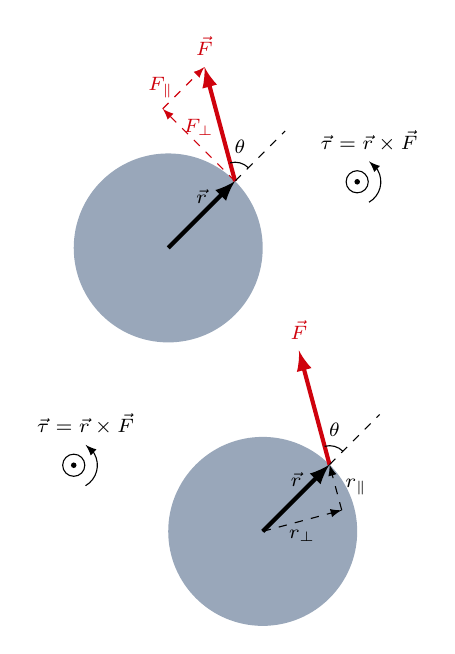
\begin{tikzpicture}[scale=1]
\tikzmath{
\R=1.2;
\Fl=1.5;
\th=60;
\Flx=\Fl*sin(\th);
\Fly=\Fl*cos(\th);
\rx=\R*sin(\th);
\ry=\R*cos(\th);
}

\scalebox{1}{

\coordinate (P) at (2*\R,0.7*\R);

\fill[myblue!40] (0,0) circle(\R);
\draw[-latex,line width=1.5] (0,0) -- (45:\R) node[midway,above]{\scriptsize $\vec r$}; 
\draw[-latex,line width=1.5,color=myred] (45:\R) -- +(45+\th: \Fl) node[above]{\scriptsize $\vec F$};
\draw[dashed] (45:\R) -- +(45:0.75*\R);
\draw (45:1.2*\R) arc(45:{45+\th}:0.2*\R) node[midway,above]{\scriptsize $\theta$};
\draw[dashed,color=myred,-latex] (45:\R) -- +(135:\Flx) node[midway,above] {\scriptsize $F_\perp$};
\draw[dashed,color=myred,-latex] ($(45:\R)+(135:\Flx)$) -- +(45:\Fly)node[midway,left] {\scriptsize $F_\parallel$};

\fill (P) circle (1pt);
\draw (P) circle (4pt);
\draw[-latex] ($(P)+(-60:0.3)$) arc (-60:60:0.3) node[above] {\scriptsize $\vec \tau = \vec r \times \vec F$};

\only<2>{
\begin{scope}[shift={(\R,-3*\R)}]
\coordinate (P2) at (-2*\R,0.7*\R);
\fill[myblue!40] (0,0) circle(\R);
\draw[-latex,line width=1.5] (0,0) -- (45:\R) node[midway,above]{\scriptsize $\vec r$}; 
\draw[-latex,line width=1.5,color=myred] (45:\R) -- +(45+\th: \Fl) node[above]{\scriptsize $\vec F$};
\draw[dashed] (45:\R) -- +(45:0.75*\R);
\draw (45:1.2*\R) arc(45:{45+\th}:0.2*\R) node[midway,above]{\scriptsize $\theta$};

\draw[dashed,-latex] (0,0) -- +(\th-45:\rx) node[midway,below] {\scriptsize $r_\perp$};
\draw[dashed,-latex] ($(0,0)+(\th-45:\rx)$) -- +(45+\th: \ry) node[midway,right] {\scriptsize $r_\parallel$};


\fill (P2) circle (1pt);
\draw (P2) circle (4pt);
\draw[-latex] ($(P2)+(-60:0.3)$) arc (-60:60:0.3) node[above] {\scriptsize $\vec \tau = \vec r \times \vec F$};
\end{scope}
}
}
\end{tikzpicture}
\captionof*{figure}{\textit{The torque from a force.}}
\end{center}
}


%%%%%%%%%%%%%%%%%%%%%%%%%%%%%%%%
\twocolframesf{Torque to rotate a door}
{
\begin{align*}
\vec \tau &= \vec r \times \vec F\\
\tau &= rF\sin\theta
\end{align*}
\begin{itemize}
\item A given force will result in the largest torque if it is perpendicular to the vector, $\vec r$ ($\sin\theta=1$).
\item A given force will result in the largest torque if the vector, $\vec r$,  has the largest magnitude.
\item That's why the door handles are far from the hinges... You knew this intuitively...
\end{itemize}
}
{
\begin{center}
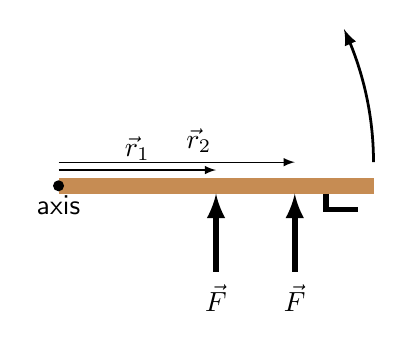
\begin{tikzpicture}[scale=1]
\tikzmath{
\L=4;
}

\scalebox{1}{

\fill[color=brown!90] (0,-0.1) rectangle (\L,0.1);
\fill (0,0) circle (2pt) node[below]{axis};
\draw[line width = 2] (0.85*\L,-0.1) -- +(0,-0.2) -- +(0.4,-.2);

\draw[latex-, line width=2] (0.5*\L,-0.1) -- +(0,-1) node[below]{$\vec F$};
\draw[latex-, line width=2] (0.75*\L,-0.1) -- +(0,-1) node[below]{$\vec F$};

\draw[-latex] (0,0.2) -- +(0.5*\L,0) node[midway,above]{$\vec r_1$};
\draw[-latex] (0,0.3) -- +(0.75*\L,0) node[midway,above right]{$\vec r_2$};

\draw [-latex, line width =1] (\L,0.3) arc (0:25:\L); 
}
\end{tikzpicture}
\captionof*{figure}{\textit{Rotating a door is easier if you push far away from the hinges, right?}}
\end{center}
}



%%%%%%%%%%%%%%%%%%%%%%%%%%%%%%%%



%%%%%%%%%%%%%%%%%%%%%%%%%%%%%%%%
\section{Angular Dynamics and Moment of Inertia}
\label{sec:angulardynamicsandmomentofinertia}
\title{Angular Dynamics and Moment of Inertia}
\institute{Describing Angular Statics and Dynamics}
\author{\insertsubsection}


%%%%%%%%%%%%%%%%%%%%%%%%%
\begin{frame}
\titlepage
\thispagestyle{empty}
\end{frame}

%%%%%%%%%%%%%%%%%%%%%%%%%





%%%%%%%%%%%%%%%%%%%%%%%%%%%%%%%%
\subsection{Dynamics of rotating objects}
\label{subsec:dynamicsofrotatingobjects}
\begin{frame}{Dynamics of rotating particles}
\begin{itemize}
\item For a point particle:
\begin{align*}
\pvec F^{net} = m\vec a
\end{align*}
\item If we choose an axis of rotation, such that, $\vec r$, is the vector from that axis to the particle:
\begin{align*}
\vec r \times \pvec F^{net} &= m\vec r \times\vec a \quad \quad \text{recall: } \vec \alpha=\frac{1}{r^2}\vec r \times \vec a\\
\therefore \pvec \tau^{net} &= mr^2\vec \alpha
\end{align*}
\item This \textbf{equation only makes sense relative to a specific axis of rotation}. It is valid even if there is nothing actually rotating!
\item The inertia of the particle to rotational motion is given by $mr^2$, and \textbf{depends on both the mass of the particle and its distance to the axis of rotation}.
\item We often refer to this as the rotational version of Newton's Second Law.
\end{itemize}
\end{frame}


%%%%%%%%%%%%%%%%%%%%%%%%%%%%%%%%



%%%%%%%%%%%%%%%%%%%%%%%%%%%%%%%%
\twocolframesf{Dynamics of rotating objects}
{
\begin{itemize}
\item We can extend the description of how one particle rotates about an axis to how a solid object rotates about an axis.
\item An object can be modeled as a ``system'' of particles, each with a torque exerted on it, and a corresponding angular acceleration:
\begin{align*}
\pvec \tau_1^{net} &= m_1r_1^2\vec \alpha_1\\
\pvec \tau_2^{net} &= m_2r_2^2\vec \alpha_2\\
&\dots
\end{align*}
\end{itemize}
}
{
\begin{center}
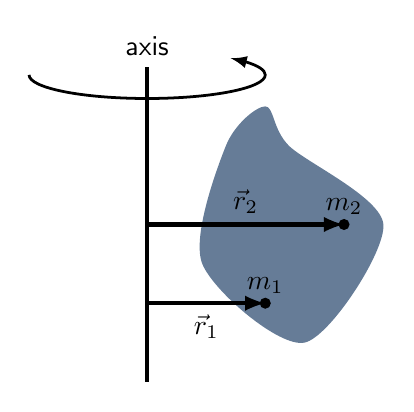
\begin{tikzpicture}[scale=1]
\tikzmath{
\L=2;
}

\scalebox{1}{

\coordinate (P1) at (1.5,-1);
\coordinate (P2) at (2.5,0);


\draw[line width=1.5] (0,-\L) -- (0,\L) node[above] {axis};

\fill[color=myblue!60] plot [smooth cycle] coordinates {(2,-1.5) (3,0) (1.8,1) (1.5,1.5) (1,1) (0.7,-0.5)};

\fill (P1) circle(2pt) node[above]{$m_1$};
\fill (P2) circle(2pt) node[above]{$m_2$};

\draw[latex-, line width=1.5] (P2) -- (0,0) node[midway,above]{$\vec r_2$};
\draw[latex-, line width=1.5] (P1) -- (0,-1) node[midway,below]{$\vec r_1$};

\draw[-latex, line width=1] (-1.5,0.95*\L) arc(-180:45:1.5 and 0.3);

}
\end{tikzpicture}
\captionof*{figure}{\textit{Two particles in a solid object rotating about an axis.}}
\end{center}
}


%%%%%%%%%%%%%%%%%%%%%%%%%%%%%%%%



%%%%%%%%%%%%%%%%%%%%%%%%%%%%%%%%
\twocolframesf{Dynamics of rotating objects}
{
\begin{itemize}
\item Rotational version of Newton’s Second Law true for each particle:
\begin{align*}
\pvec \tau_1^{net} &= m_1r_1^2\vec \alpha_1\\
\pvec \tau_2^{net} &= m_2r_2^2\vec \alpha_2\\
&\dots
\end{align*}
\item Sum these all together:
\begin{itemize}
\item \textbf{All particles have the same angular acceleration}.
\item When summing the torques on each particle, all of the internal torques (due to internal forces) cancel:
\begin{align*}
\sum \pvec \tau^{ext}=\left(\sum m_ir_i^2  \right)\vec \alpha
\end{align*}
\end{itemize}

\end{itemize}
}
{
\begin{center}
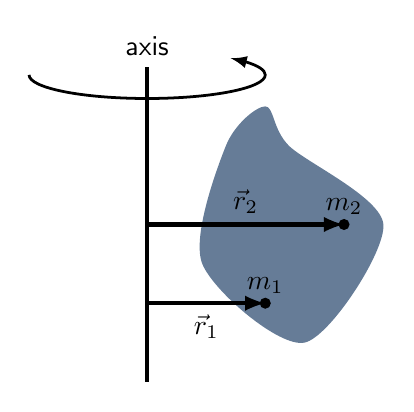
\begin{tikzpicture}[scale=1]
\tikzmath{
\L=2;
}

\scalebox{1}{

\coordinate (P1) at (1.5,-1);
\coordinate (P2) at (2.5,0);


\draw[line width=1.5] (0,-\L) -- (0,\L) node[above] {axis};

\fill[color=myblue!60] plot [smooth cycle] coordinates {(2,-1.5) (3,0) (1.8,1) (1.5,1.5) (1,1) (0.7,-0.5)};

\fill (P1) circle(2pt) node[above]{$m_1$};
\fill (P2) circle(2pt) node[above]{$m_2$};

\draw[latex-, line width=1.5] (P2) -- (0,0) node[midway,above]{$\vec r_2$};
\draw[latex-, line width=1.5] (P1) -- (0,-1) node[midway,below]{$\vec r_1$};

\draw[-latex, line width=1] (-1.5,0.95*\L) arc(-180:45:1.5 and 0.3);

}
\end{tikzpicture}
\captionof*{figure}{\textit{The particles in a solid object rotating about an axis all have the same angular acceleration relative to that axis.}}
\end{center}
}


%%%%%%%%%%%%%%%%%%%%%%%%%%%%%%%%
\subsection{Moment of inertia}
\label{subsec:momentofinertia}
\begin{frame}{The moment of inertia}
\begin{itemize}
\item The net external torque on an object determines its angular acceleration:
\begin{align*}
\sum \pvec \tau^{ext}=\left(\sum m_ir_i^2  \right)\vec \alpha
\end{align*}
\item We introduce, $I$, the ``moment of inertia'' of an object \textbf{relative to a given axis of rotation}:
\begin{align*}
I=\sum m_ir_i^2  
\end{align*}
\item Rotational version of Newton's Second Law:
\begin{align*}
\sum \pvec \tau^{ext}=I\vec \alpha
\end{align*}
\item Instead of force, we have torque, instead of mass, we have moment of inertia, instead of linear acceleration, we have angular acceleration.
\end{itemize}
\end{frame}


%%%%%%%%%%%%%%%%%%%%%%%%%%%%%%%%
\begin{frame}{Rotational vs Linear dynamics}
\begin{itemize}
\item Recall, for an object, the \textbf{net external force} on the object determines \textbf{the acceleration of the CM}:
\begin{align*}
\sum \pvec F^{ext}=M\vec a_{CM}
\end{align*}
\item Similarly, the \textbf{net external torque} about an axis on the object determines its \textbf{angular acceleration} relative to that axis:
\begin{align*}
\text{cause of motion}\quad\quad\sum \pvec \tau^{ext}=I\vec \alpha\quad\quad\text{(resistance to motion)(kinematic quantity)}
\end{align*}
\item The moment of inertia has a similar ``role'' as the mass in Newton's Second Law. For a given torque, the object with the smaller moment of inertia will have the largest angular acceleration.
\end{itemize}
\end{frame}



%%%%%%%%%%%%%%%%%%%%%%%%%%%%%%%%
\subsection{Group exercise: moment of inertia for a 2 mass system}
\label{subsec:}
\twocolframesf{Group exercise}
{
\begin{itemize}
\item Calculate the moment of inertia for a system of 2 masses connected by a mass-less rod of length $d$, for:
\begin{itemize}
\item An axis that goes through $m_1$.
\item An axis that goes through 0 ($d$ away from $m_1$).
In both cases, the axis is perpendicular to the page.
\end{itemize}
\begin{align*}
I=\sum m_ir_i^2  
\end{align*}
\item<2> Applying the formula:
\begin{align*}
I_{m_1}&=m_1(0)^2+m_2d^2=m_2d^2\\
I_{0}&=m_1(d)^2+m_2(2d)^2=(m_1+4m_2)d^2\\
\end{align*}
\end{itemize}
}
{
\begin{center}
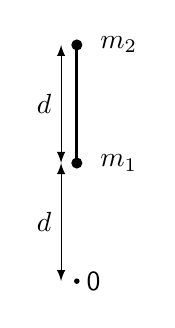
\begin{tikzpicture}[scale=1]
\tikzmath{
\d=1.5;
}

\scalebox{1}{

\fill (0,0) circle (1pt) node[right] {0};
\fill (0,\d) circle (2pt) node[right=5pt] {$m_1$};
\fill (0,2*\d) circle (2pt) node[right=5pt] {$m_2$};
\draw[latex-latex] (-0.2,0) -- +(0,\d) node[midway, left]{$d$};
\draw[latex-latex] (-0.2,\d) -- +(0,\d) node[midway, left]{$d$};
\draw[line width=1] (0,\d) -- +(0,\d);
}
\end{tikzpicture}
\captionof*{figure}{\textit{Two masses connected by a mass-less rods rotate around an axis perpendicular to the page.}}
\end{center}
}


%%%%%%%%%%%%%%%%%%%%%%%%%%%%%%%%



%%%%%%%%%%%%%%%%%%%%%%%%%%%%%%%%
\subsection{Formula}
\label{subsec:iformula}
\begin{frame}{Calculating moment of inertia}
\begin{itemize}
\item Similar to centre of mass, which is a mass-weighted sum of the position coordinate:
\begin{align*}
x_{CM}=\frac{1}{M}\sum m_ix_i=\frac{1}{M}\int_0^M xdm
\end{align*}
\item For the moment of inertia, it is a mass-weighted sum of the \textbf{distance to the axis of rotation squared}:
\begin{align*}
I=\sum m_ir_i^2  =\int_0^M r^2 dm
\end{align*}
\end{itemize}
\end{frame}


%%%%%%%%%%%%%%%%%%%%%%%%%%%%%%%%
\subsection{Example: moment of inertia of a rod about its end}
\label{subsec:}
\twocolframesf{Continuous objects: Moment of inertia of a rod about its end}
{
\begin{itemize}
\item Define mass per unit length: $\lambda =\frac{M}{L}$
\item Choose a mass element on the rod, $dm$, of length, $dr$ , at a distance, $r$, from the axis of rotation, it has mass:
\begin{align*}
dm=\lambda dr
\end{align*}
\item The total moment of inertia is the sum over all mass elements:
\begin{align*}
I_{end}&=\sum m_ir_i^2  =\int_0^M r^2 dm = \int_0^L \lambda r^2 dr\\
&=\lambda \frac{1}{3}L^3=\frac{1}{3}ML^2
\end{align*}
\end{itemize}
}
{
\begin{center}
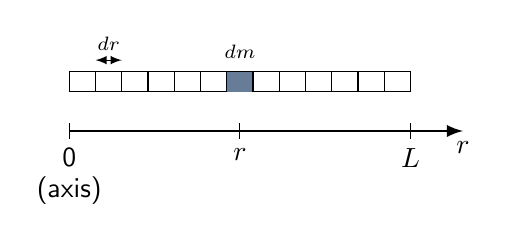
\begin{tikzpicture}
\tikzmath{
\L=5;
\n=15;
}
\scalebox{1}{

\draw[-latex,line width=1] (0,0) -- (\L,0) node[below]{$r$};
\draw (0,0.1) -- +(0,-0.2) node[below]{0} node[below=10pt]{(axis)};
\draw (\L/\n*13,0.1) -- +(0,-0.2) node[below]{$L$};


\foreach \i in {1,...,13}{
\tikzmath{
\dx=\L/\n;
\xxi=\dx*(\i-1);
}
\draw (\xxi,0.5) rectangle (\xxi+\dx,0.75);
\ifthenelse{\i=7}{
\fill[color=myblue!60] (\xxi,0.5) rectangle (\xxi+\dx,0.75);
\node at (\xxi+0.5*\dx,1) {\scriptsize $dm$};
\draw (\xxi+0.5*\dx,0.1) -- +(0,-0.2) node[below]{$r$};
}{}

\ifthenelse{\i=2}{
\draw[latex-latex] (\xxi,0.9) -- +(0\dx,0) node[midway,above]{\scriptsize $dr$};
}{}

}


}
\end{tikzpicture}
\captionof*{figure}{\textit{To find the moment of inertia of a one dimensional object, model it as being made of many \textit{point} masses, $dm$, each with an infinitesimal length, $dx$.}}
\end{center}
}


%%%%%%%%%%%%%%%%%%%%%%%%%%%%%%%%
\begin{frame}{Group exercise}
Determine the moment of inertia of a uniform rod about is centre of mass:
\begin{itemize}
\item Do you expect it to be bigger or smaller than moment of inertia about its end?
\end{itemize}
\end{frame}


%%%%%%%%%%%%%%%%%%%%%%%%%%%%%%%%
\twocolframesf{Continuous objects: Moment of inertia of a rod about its end}
{
\begin{itemize}
\item Define mass per unit length: $\lambda =\frac{M}{L}$
\item Choose a mass element on the rod, $dm$, of length, $dr$ , at a distance, $r$, from the axis of rotation, it has mass:
\begin{align*}
dm=\lambda dr
\end{align*}
\item The total moment of inertia is the sum over all mass elements:
\begin{align*}
I_{CM}&=\sum m_ir_i^2  =\int_0^M r^2 dm = \int_{\textcolor{myred}{-\frac{L}{2}}}^{\textcolor{myred}{+\frac{L}{2}}} \lambda r^2 dr\\
&=\lambda \left[\frac{1}{3}r^3\right]_{\textcolor{myred}{-\frac{L}{2}}}^{\textcolor{myred}{+\frac{L}{2}}} =\frac{1}{12}\lambda ML^3=\frac{1}{12}ML^2
\end{align*}
\end{itemize}
}
{
\vspace{-0.5cm}
\begin{center}
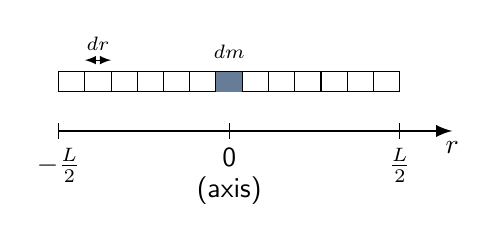
\begin{tikzpicture}
\tikzmath{
\L=5;
\n=15;
}
\scalebox{1}{

\draw (0,0.1) -- +(0,-0.2) node[below]{$-\frac{L}{2}$};
\draw[-latex,line width=1] (0,0) -- (\L,0) node[below]{$r$};
\draw (\L/\n*13,0.1) -- +(0,-0.2) node[below]{$\frac{L}{2}$};


\foreach \i in {1,...,13}{
\tikzmath{
\dx=\L/\n;
\xxi=\dx*(\i-1);
}
\draw (\xxi,0.5) rectangle (\xxi+\dx,0.75);
\ifthenelse{\i=7}{
\fill[color=myblue!60] (\xxi,0.5) rectangle (\xxi+\dx,0.75);
\node at (\xxi+0.5*\dx,1) {\scriptsize $dm$};
%\draw (\xxi+0.5*\dx,0.1) -- +(0,-0.2) node[below]{$r$};
\draw (\xxi+0.5*\dx,0.1) -- +(0,-0.2) node[below]{0} node[below=10pt]{(axis)};
}{}

\ifthenelse{\i=2}{
\draw[latex-latex] (\xxi,0.9) -- +(0\dx,0) node[midway,above]{\scriptsize $dr$};
}{}

}


}
\end{tikzpicture}
\captionof*{figure}{\textit{To find the moment of inertia of a rod about CM, we move the origin to the axis of rotation, so that $r$ measures distance to the axis.}}
\end{center}
Alternatively, we could have added the moment of inertia of two rods of length $\frac{1}{2}L$ (and mass $\frac{M}{2}$) rotated about their ends:
\begin{align*}
I_{CM}&=2\frac{1}{3}\frac{M}{2}\left(\frac{L}{2} \right)^2=\frac{1}{12}ML^2
\end{align*}
}



%%%%%%%%%%%%%%%%%%%%%%%%%%%%%%%%
\subsection{Parallel axis theorem}
\label{subsec:parallelaxistheorem}
\twocolframesf{Parallel axis theorem}
{
\begin{itemize}
\item Given the moment of inertia about an axis that goes through the CM, the moment of inertia about an axis that is parallel and goes through a different point, a distance, $h$ away is given by:
\begin{align*}
I_h=I_{CM}+Mh^2
\end{align*}
\item For a rod, find the moment of inertia about the CM, given the moment of inertia about one end:
\begin{align*}
I_{end}&=\frac{1}{3}ML^2\\
I_{CM}&=I_{end}-M\left(\frac{L}{2}\right)^2=\frac{1}{3}ML^2-\frac{1}{4}ML^2=\frac{1}{12}ML^2
\end{align*}
\end{itemize}
}
{
\vspace{-0.5cm}
\begin{center}
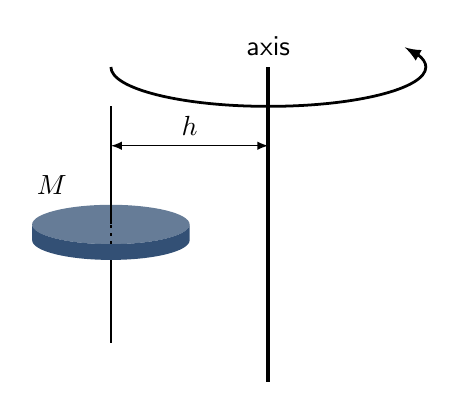
\begin{tikzpicture}
\tikzmath{
\R=1;
\h=2;
\L=4;
}
\scalebox{1}{

\node at (-0.75*\R,0.5*\R){$M$};
\fill[color=myblue!60] circle ({\R} and {\R/4});
\draw[line width=1] (0,0) -- +(0,0.75*\L/2);
\draw[line width=1] (0,-0.75*\L/2) -- (0,-\R/4);
\draw[line width=1, dotted] (0,-\R/4) -- (0,0);
\fill[color=myblue!80] (\R,0) arc(0:-180:{\R} and {\R/4}) -- (-\R,-0.2) arc(180:360:{\R} and {\R/4}) -- cycle;

\draw[line width=1.5] (\h,-\L/2) -- +(0,\L)node[above]{axis};
\draw[latex-latex] (0,\L/4) -- +(\h,0)node[midway,above]{$h$} ;

\draw[-latex,line width=1] (0,\L/2) arc(180:390:{\h} and {\h/4});

}
\end{tikzpicture}
\captionof*{figure}{\textit{The moment of inertia of an object about an axis a distance, $h$, away from the CM is given by the parallel axis theorem.}}
\end{center}

}

%%%%%%%%%%%%%%%%%%%%%%%%%%%%%%%%

%%%%%%%%%%%%%%%%%%%%%%%%%%%%%%%%%%%%%%

\begin{frame}{Quick review}
\subsection{Review}
\label{subsec:review}
\begin{itemize}
\item Torque from a force \textbf{about an axis}:
\begin{align*}
\vec \tau =\vec r \times \vec F
\end{align*}
\item Rotational equivalent of Newton's Second Law:
\begin{align*}
\pvec \tau^{net}&=mr^2\vec \alpha\quad \text{(particle)}\\
\sum \pvec \tau^{ext}&=I\vec \alpha\quad \text{(object)}
\end{align*}
\item Moment of inertia of an object \textbf{about an axis}:
\begin{align*}
I=\sum m_ir_i^2  =\int_0^M r^2 dm
\end{align*}
\item Parallel axis theorem:
\begin{align*}
I_h=I_{CM}+Mh^2
\end{align*}
\end{itemize}
\end{frame}

%%%%%%%%%%%%%%%%%%%%%%%%%%








%%%%%%%%%%%%%%%%%%%%%%%%%%%%%%%%
\section{Equilibriem with Rotational Dynamics}
\label{sec:equilibirem}
\title{quilibriem with Rotational Dynamics}
\institute{Describing Angular Statics and Dynamics}
\author{\insertsubsection}


%%%%%%%%%%%%%%%%%%%%%%%%%
\begin{frame}
\titlepage
\thispagestyle{empty}
\end{frame}

%%%%%%%%%%%%%%%%%%%%%%%%%





%%%%%%%%%%%%%%%%%%%%%%%%%%%%%%%%
\subsection{Concept}
\label{subsec:concept}
\twocolframe{Equilibrium}
{
\begin{itemize}
\item Just because the sum of the external forces on an object is zero does not mean that the object does not move. It only means that the centre of mass does not accelerate:
\begin{align*}
\sum \pvec F^{ext}=m\vec a_{CM}
\end{align*}
\item For the object to be ``in equilibrium'' the sum of the torques on the object must also be zero:
\begin{align*}
\sum \pvec \tau^{ext}=I\vec \alpha
\end{align*}
\end{itemize}

}
{
\begin{center}
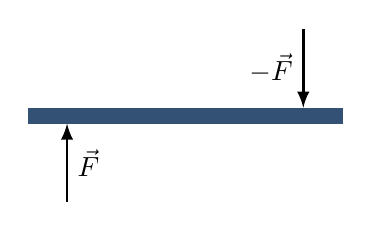
\begin{tikzpicture}[scale=1]
\tikzmath{
\L=2;
}

\scalebox{1}{
\fill[color=myblue!80] (-\L,-0.1) rectangle (\L,0.1);
\draw[latex-,line width=1] (-0.75*\L,-0.1) -- +(0,-1) node[midway,right] {$\vec F$};
\draw[latex-,line width=1] (0.75*\L,0.1) -- +(0,1) node[midway,left] {$-\vec F$};
}
\end{tikzpicture}
\captionof*{figure}{\textit{The net force on this bar is zero, but it will rotate because the net torque (about any axis!) is not zero. }}
\end{center}
}


%%%%%%%%%%%%%%%%%%%%%%%%%%%%%%%%


%%%%%%%%%%%%%%%%%%%%%%%%%%%%%%%%

%%%%%%%%%%%%%%%%%%%%%%%%%%%%%%%%
\twocolframe{Equilibrium}
{
\begin{itemize}
\item Just because the sum of the external forces on an object is zero does not mean that the object does not move. It only means that the centre of mass does not accelerate:
\begin{align*}
\sum \pvec F^{ext}=m\vec a_{CM}
\end{align*}
\item For the object to be ``in equilibrium'' the sum of the torques \textcolor{myred}{about any axis} on the object must also be zero:
\begin{align*}
\sum \pvec \tau^{ext}=I\vec \alpha
\end{align*}
\end{itemize}

}
{
\begin{center}
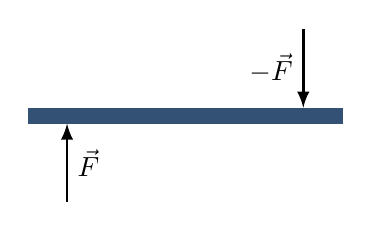
\begin{tikzpicture}[scale=1]
\tikzmath{
\L=2;
}

\scalebox{1}{
\fill[color=myblue!80] (-\L,-0.1) rectangle (\L,0.1);
\draw[latex-,line width=1] (-0.75*\L,-0.1) -- +(0,-1) node[midway,right] {$\vec F$};
\draw[latex-,line width=1] (0.75*\L,0.1) -- +(0,1) node[midway,left] {$-\vec F$};
}
\end{tikzpicture}
\captionof*{figure}{\textit{The net force on this bar is zero, but it will rotate because the net torque is not zero. Note that it will rotate about the CM because that is the point that behaves according to the net external force, which is zero, so the CM does not move!}}
\end{center}
}


%%%%%%%%%%%%%%%%%%%%%%%%%%%%%%%%



%%%%%%%%%%%%%%%%%%%%%%%%%%%%%%%%
\subsection{Example: ladder}
\label{subsec:exampleladder}
\twocolframesf{Example: ladder}
{
\only<1>{
\begin{itemize}
\item Group question: Draw the forces on the ladder.
\end{itemize}
}
\only<2>{
\begin{itemize}
\item The friction force on the ground prevents the bottom of the ladder from sliding away.
\item If you consider the torques about the contact point with the ground, the torque on the ladder from the weight of the person on the ladder gets bigger as they climb up:
\begin{itemize}
\item Only $R$ can grow and exert a torque in the opposite direction to keep the ladder in equilibrium.
\item As $R$ increases, $f_s$ must also increase (not net force in the horizontal direction).
\end{itemize}
\item When someone ``spots you'' on a ladder, the most important is that they prevent the bottom of the ladder from sliding away from the wall.

\end{itemize}
}
}
{
\begin{center}
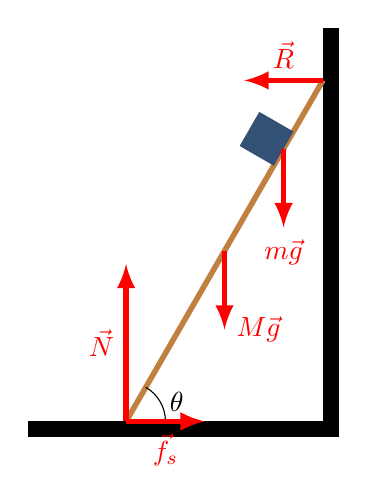
\begin{tikzpicture}[scale=1]
\tikzmath{
\L=5;
\abox=0.5;
\th=60;
\xl=0.5*\L;
\ladl=\xl/cos(\th);
}

\scalebox{1}{
\coordinate (P) at (-\xl,0);
\coordinate (R) at ($(P)+(\th:\ladl)$);
\coordinate (B) at ($(P)+(\th:0.75*\ladl)$);

\fill (-0.75*\L,-0.2) rectangle (0,0);
\fill (0,-0.2) rectangle (0.2,1*\L);

\draw[line width=2,color=brown] (P) -- (R);
\draw ($(P)+(0.5,0)$) arc(0:\th:0.5) node[midway,right]{$\theta$};

\begin{scope}[rotate=\th]
\fill[color=myblue!80] (B) -- ($(B)+(0:\abox)$) -- ($(B)+(0:\abox)+(90:\abox)$)-- ($(B)+(90:\abox)$) -- cycle;
\end{scope}

\only<2>{
\draw[-latex,color=red,line width=2] (P) -- +(0,2) node[midway,left]{$\vec N$};
\draw[-latex,color=red,line width=2] (P) -- +(1,0) node[midway,below]{$\vec f_s$};

\draw[-latex,color=red,line width=2] ($(P) +(\th:0.5*\ladl)$) -- +(0,-1)node[right]{$M\vec g$};
\draw[-latex,color=red,line width=2] ($(P) +(\th:0.75*\ladl+\abox/2)$) -- +(0,-1)node[below]{$m\vec g$};

\draw[-latex,color=red,line width=2] (R) -- +(-1,0) node[midway,above]{$\vec R$};


}

}
\end{tikzpicture}
\only<1>{\captionof*{figure}{\textit{A ladder with a weight on it.}}}
\only<2>{\captionof*{figure}{\textit{Forces exerted \textbf{on the ladder}.}}}
\end{center}
}


%%%%%%%%%%%%%%%%%%%%%%%%%%%%%%%%
\twocolframe{Ladder safety: which is safest (from a statics perspective)?}
{
\capfig{0.7}{../figures/RotationalDynamics/ladder1}{}
}
{
\capfig{1}{../figures/RotationalDynamics/ladder2}{}
}


%%%%%%%%%%%%%%%%%%%%%%%%%%%%%%%%
\subsection{CM of irregular shapes}
\label{subsec:cmofirregularshapes}
\twocolframe{Example: Find CM of object}
{
\begin{itemize}
\item Only two forces on the object:
\begin{itemize}
\item Weight \textbf{exerted at the CM}.
\item Normal force exerted by the pin.
\end{itemize}
\item Since the object is in equilibrium, there is no net torque.
\item The CM must be located exactly below the pin, or the weight and normal force would create a net torque.
\end{itemize}
}
{
\begin{center}
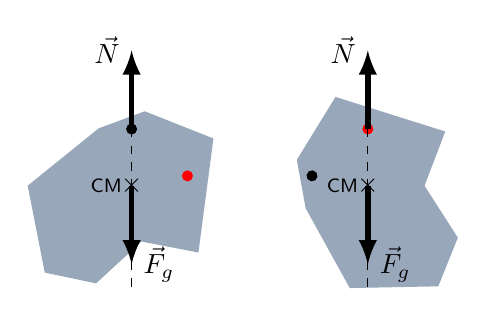
\begin{tikzpicture}[scale=1]
\tikzmath{
\th=80;
\L=1.2;
}

\scalebox{1}{

\coordinate (CM) at (0,0);

\fill[color=myblue!40] ($(CM)+(80:0.8*\L)$) -- ($(CM)+(30:\L)$) -- ($(CM)+(-45:\L)$)  -- ($(CM)+(-80:0.6*\L)$) -- ($(CM)+(250:1.1*\L)$) -- ($(CM)+(225:1.3*\L)$) -- ($(CM)+(180:1.1*\L)$) -- ($(CM)+(120:0.7*\L)$) -- cycle;

\fill ($(CM)+(0,0.6*\L)$) circle(2pt);
\fill[color=red] ($(CM)+(10:0.6*\L)$) circle(2pt);
\draw[-latex,line width=2] ($(CM)+(0,0.6*\L)$) --+(0,1) node[left]{$\vec N$};
\draw[dashed] ($(CM)+(0,0.6*\L)$) --+(0,-2);
\draw[-latex,line width=2] ($(CM)$) --+(0,-1) node[right]{$\vec F_g$};
\node at (CM) {$\times$};
\node[left] at (CM) {\scriptsize CM};


\begin{scope}[shift={(2.5*\L,0)}]

\coordinate (CM) at (0,0);
\begin{scope}[rotate=\th]
\fill[color=myblue!40] ($(CM)+(80:0.8*\L)$) -- ($(CM)+(30:\L)$) -- ($(CM)+(-45:\L)$)  -- ($(CM)+(-80:0.6*\L)$) -- ($(CM)+(250:1.1*\L)$) -- ($(CM)+(225:1.3*\L)$) -- ($(CM)+(180:1.1*\L)$) -- ($(CM)+(120:0.7*\L)$) -- cycle;
\fill ($(CM)+(0,0.6*\L)$) circle(2pt);
\end{scope}


\fill[color=red] ($(CM)+(\th+10:0.6*\L)$) circle(2pt);
\draw[-latex,line width=2] ($(CM)+(10+\th:0.6*\L)$) --+(0,1) node[left]{$\vec N$};
\draw[dashed] ($(CM)+(10+\th:0.6*\L)$) --+(0,-2);
\draw[-latex,line width=2] ($(CM)$) --+(0,-1) node[right]{$\vec F_g$};
\node at (CM) {$\times$};
\node[left] at (CM) {\scriptsize CM};

\end{scope}

}
\end{tikzpicture}
\captionof*{figure}{\textit{Rotating a 2D shape and using a plumbline to find its CM. The CM corresponds to the location where the net force of gravity is exerted, sometimes called the ``centre of gravity''.}}
\end{center}
}


%%%%%%%%%%%%%%%%%%%%%%%%%%%%%%%%



%%%%%%%%%%%%%%%%%%%%%%%%%%%%%%%%
\subsection{Dynamics cs static equilibriem}
\label{subsec:dynamicsvsstaticequilibriem}
\begin{frame}{Dynamic vs Static equilibrium}
\begin{itemize}
\item Equilibrium $\rightarrow$ Sum of the torques is zero.
\item Static equilibrium $\rightarrow$ The net force is zero (the CM does not accelerate).
\item Dynamic equilibrium $\rightarrow$ The net force is not zero (the CM accelerates, as does any axis of rotation that is ``attached'' to the object).
\end{itemize}
\end{frame}


%%%%%%%%%%%%%%%%%%%%%%%%%%%%%%%%
\subsection{Speed skater example}
\label{subsec:speed skater example}
\twocolframe{Speed skater in dynamic equilibrium}
{
\only<1>{
\begin{itemize}
\item The skater is accelerating to the left (going around a curve, centre of the circle is to the left).
\item The skater is \textbf{not} rotating about her CM!
\begin{itemize}
\item The torques from the normal force and the friction force cancel.
\end{itemize}
\item However, taking the torques about the bottom point, we find there is a net torque from gravity. What is going on?
\end{itemize}

}
\only<2>{
\begin{itemize}
\item The sum of torques about the bottom point is not zero! Why?
\begin{itemize}
\item The accelerating skater is a \textbf{non-inertial frame of reference}. The \textbf{bottom point corresponds to an axis that is accelerating} with the skater.
\item You can take the torques about the bottom point if you consider \textbf{inertial forces}.
\item You \textbf{can always take the torques about the CM}, because the inertial force exerted at the CM will result in no torque, so it won’t matter if the CM is accelerating.
\end{itemize}
\end{itemize}
}
}
{
\vspace{-0.75cm}
\begin{center}
\begin{tikzpicture}[scale=1]
\tikzmath{
\h=2.5;
\L=3;
}

\scalebox{1}{
\node at (0,\h){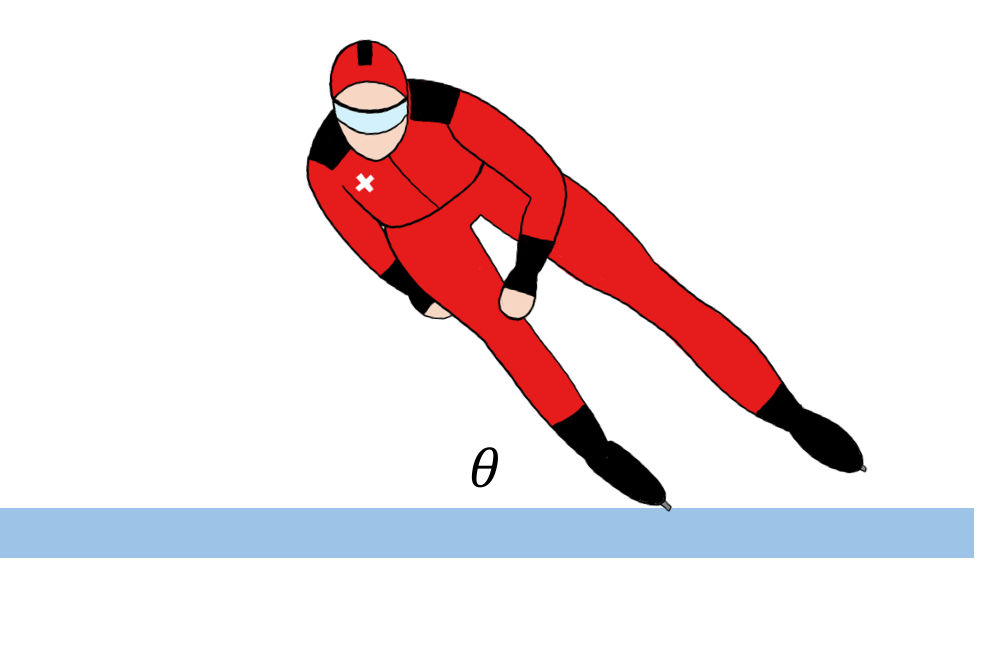
\includegraphics[scale=0.3]{../figures/RotationalDynamics/skater}};

\draw [line width=3,color=red] (135:\L/2) -- (-45:\L/2);
\fill (0,0) circle (2pt) node[below left]{\scriptsize CM};
\draw [-latex,line width=2] (0,0) -- +(0,-1) node[left]{$\vec F_g$};
\draw [-latex,line width=2] (-45:\L/2) -- +(0,1) node[right]{$\vec N$};
\draw [-latex,line width=2] (-45:\L/2) -- +(-0.75,0) node[below]{$\vec f_s$};
\only<1>{
\draw [-latex,line width=3] (-0.3*\L,0) -- +(-1,0) node[below]{$\vec a_{CM}$};
}
\only<2>{
\draw [-latex,line width=2] (0,0) -- +(0.75,0) node[above]{$-m\vec a_{CM}$};
}
}
\end{tikzpicture}
\only<1>{\captionof*{figure}{\textit{Forces on a speed skater, as viewed from the ground.}}}
\only<2>{\captionof*{figure}{\textit{Forces on a speed skater, as viewed from a reference frame accelerating with the skater. You need to include inertial forces if taking torques in an accelerating frame of reference!}}}
\end{center}
}


%%%%%%%%%%%%%%%%%%%%%%%%%%%%%%%%


%%%%%%%%%%%%%%%%%%%%%%%%%%%%%%%%
\subsection{Car going around a curve}
\label{subsec:cargoingaroundacurve}
\twocolframesf{Car going around a curve}
{
\begin{itemize}
\item The friction forces, $\vec f_s$, from the tires, perpendicular to the direction of motion, provide the ``centripetal force'' (the net force towards the centre of the circle).
\item These create a net torque about the CM of the car.
\item The car leans to the left (and compresses the shocks which provide the counter torque).
\end{itemize}
}
{
\begin{center}
\begin{tikzpicture}[scale=1]
\tikzmath{
\L=4;
\h=3;
}

\scalebox{1}{
\node at (0,\h) {
\includegraphics[scale=1.2]{../figures/RotationalDynamics/car}};
\draw[-latex, line width=1.5] (0.85,0.77*\h) -- +(1,0) node[below]{$\vec f_{s1}$};
\draw[-latex, line width=1.5] (-0.98,0.77*\h) -- +(1.2,0) node[below]{$\vec f_{s2}$};
\draw[-latex, line width=3] (1.2,1*\h) -- +(1.5,0) node[midway,above]{$\vec a_{CM}$};

\node at (0,0) {\animategraphics[autoplay,loop,width=4cm]{10}{../figures/RotationalDynamics/cornering}{1}{19}};
}
\end{tikzpicture}
\captionof*{figure}{\textit{Forces on a cornering car.}}
\end{center}
}

%%%%%%%%%%%%%%%%%%%%%%%%%%%%%%%%
\subsection{Braking}
\label{subsec:braking}
\begin{frame}{Braking}
\vspace{-1cm}
\begin{center}
\begin{tikzpicture}[scale=1]
\tikzmath{
}

\scalebox{1}{
\node at (0,0) {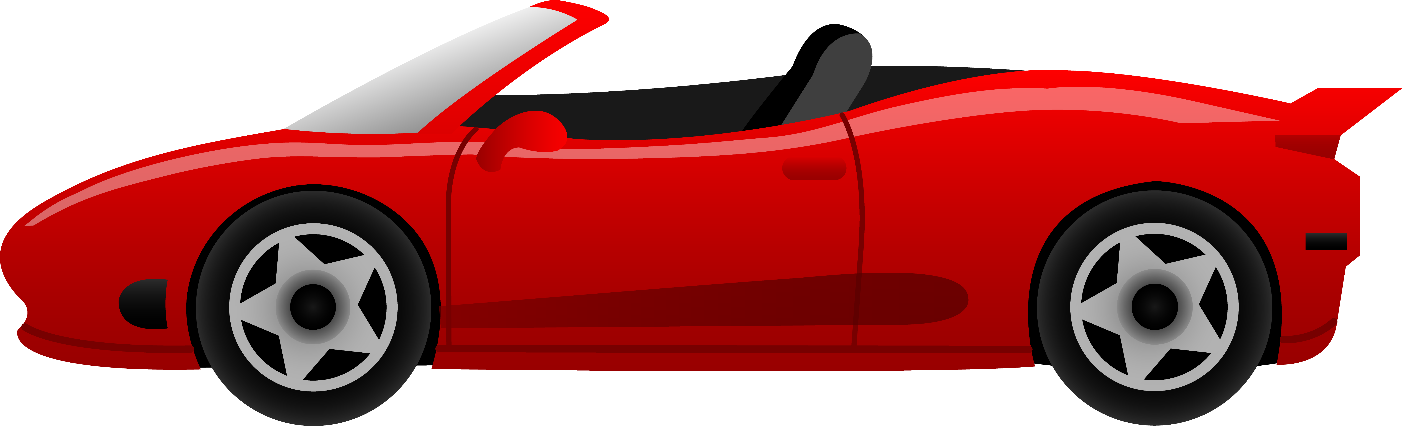
\includegraphics[scale=0.4]{../figures/RotationalDynamics/racecar}};
\draw[-latex, line width=1.5] (2.1,-0.97) -- +(1,0) node[below]{$\vec f_{s1}$};
\draw[-latex, line width=1.5] (-1.8,-0.97) -- +(2,0) node[below]{$\vec f_{s2}$};

\node at (6.5,1.75) {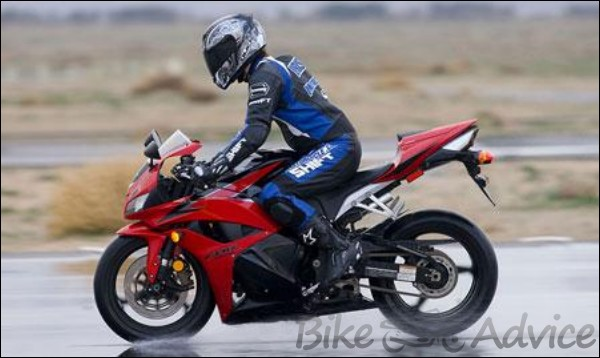
\includegraphics[scale=0.7]{../figures/RotationalDynamics/bike}};
\node at (6.5,-0.65) {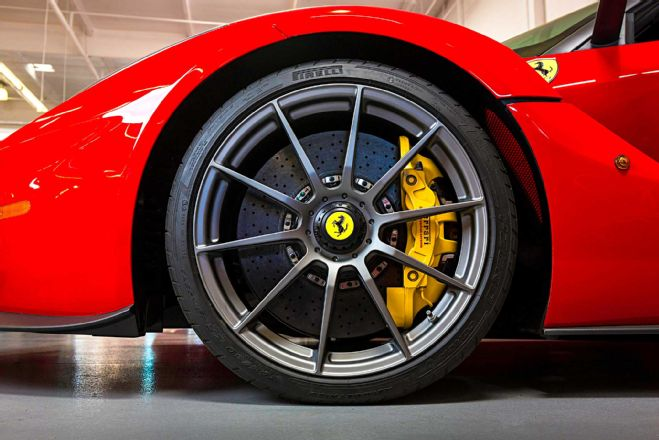
\includegraphics[scale=0.15]{../figures/RotationalDynamics/ferrari}};
}
\end{tikzpicture}
\captionof*{figure}{\textit{Due to the torque from the braking wheels and resulting normal force, the front wheel(s) do most of the braking}}
\end{center}


\begin{itemize}
\item The friction forces from the tires provide the force to decelerate.
\item The front of the car goes down because of the net torque about the CM of the car.
\item The normal force is greater at the front, the front wheels do most of the breaking! Look at the breaks in a car/motorcycle: they are \textit{way} bigger on the front wheels!
\end{itemize}
\end{frame}

%%%%%%%%%%%%%%%%%%%%%%%%%%%%%%%%



%%%%%%%%%%%%%%%%%%%%%%%%%%%%%%%%



%%%%%%%%%%%%%%%%%%%%%%%%%%%%%%%%



%%%%%%%%%%%%%%%%%%%%%%%%%%%%%%%%



%%%%%%%%%%%%%%%%%%%%%%%%%%%%%%%%



%%%%%%%%%%%%%%%%%%%%%%%%%%%%%%%%



%%%%%%%%%%%%%%%%%%%%%%%%%%%%%%%%



%%%%%%%%%%%%%%%%%%%%%%%%%%%%%%%%



%%%%%%%%%%%%%%%%%%%%%%%%%%%%%%%%



%%%%%%%%%%%%%%%%%%%%%%%%%%%%%%%%



%%%%%%%%%%%%%%%%%%%%%%%%%%%%%%%%



%%%%%%%%%%%%%%%%%%%%%%%%%%%%%%%%



%%%%%%%%%%%%%%%%%%%%%%%%%%%%%%%%






\end{document}



